\documentclass[conference]{IEEEtran}
\usepackage[utf8]{inputenc}
\usepackage{amsmath}
\usepackage{amsfonts}
\usepackage{amssymb}
\usepackage{graphicx}
\usepackage{cite}
\usepackage{url}
\usepackage{hyperref}
\usepackage{tabularx}
\usepackage{tikz}
\usepackage{makecell}
\usetikzlibrary{shapes.multipart, arrows.meta, positioning}
\urlstyle{same}
\IEEEpeerreviewmaketitle

\title{WORKING DRAFT: Multi-Objective Optimization for Automated Guitar Tablature: The gtrsnipe Fretboard Mapper}

\author{
\IEEEauthorblockN{Scott VanRavenswaay}
\IEEEauthorblockA{Email: scottvr@gmail.com}
}

\begin{document}

\maketitle

\begin{abstract}
The task of transcribing music for fretted string instruments like the guitar presents a significant computational challenge known as the \emph{fretboard mapping problem}. For any given musical pitch, multiple string–fret combinations may exist, leading to a combinatorial explosion of potential fingerings for a sequence of notes. This paper introduces the gtrsnipe Fretboard Mapper, a novel system that frames this problem as a multi-objective optimization task. The system employs a configurable, weighted scoring function that evaluates candidate fingerings based on physical playability, ergonomic efficiency, and musical context. Key components of the scoring model include penalties for wide fret stretches, excessive hand movement, and frequent string switching, along with bonuses for exploiting instrument-specific affordances such as open strings, barre chords, and ringing sustain. The mapper also incorporates a context-aware algorithm that considers previous fingerings to ensure smooth transitions, and a rule-based system for inferring performance techniques such as hammer-ons, pull-offs, and taps. We show that this multi-objective approach produces tablature that is not only playable, but also stylistically and ergonomically coherent, representing a significant improvement over naive or rule-based systems.

\end{abstract}

\begin{IEEEkeywords}
Music Information Retrieval, Guitar Tablature, Multi-Objective Optimization, Fretboard Mapping, Music Transcription, Automated Transcription
\end{IEEEkeywords}

\section{Introduction}

Music Information Retrieval (MIR) has made significant strides in automated music transcription, particularly in converting audio signals to a symbolic representation like MIDI (Musical Instrument Digital Interface). However, for multi-timbral instruments like the guitar, a MIDI representation is only an intermediate step. The core challenge lies in mapping the abstract pitches of a MIDI event sequence onto the physical constraints of the guitar's fretboard. This is a non-trivial problem due to the instrument's inherent ambiguity.

Unlike a piano, where each pitch corresponds to a single key, a standard-tuned 6-string guitar can produce the same pitch in up to six different locations. For example, the note E4 can be played as the open 1st string, or as the 5th, 9th, or 14th fret on progressively lower-pitched strings. A three-note chord can therefore have dozens of potential fingerings, or voicings. The task of an automated tablature system is to select the single ``best'' fingering for each moment in the music from this vast search space.

This paper details the gtrsnipe Fretboard Mapper, an algorithmic solution to this problem. The system extends beyond naive, greedy approaches by implementing a context-aware scoring function that models the decision-making process of a human guitarist. It balances multiple, often competing, objectives to generate tablature that is both technically feasible and musically coherent.

\begin{figure}[htbp]
\centering
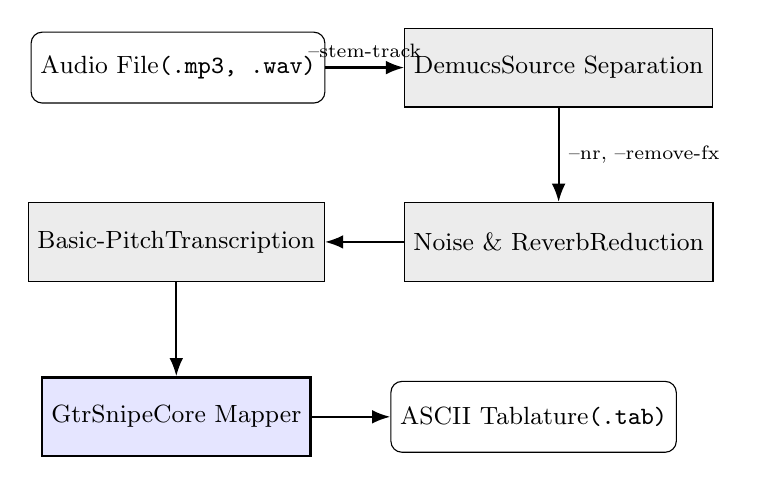
\begin{tikzpicture}[
  node distance=1.2cm and 1.0cm,
  every node/.style={font=\small},
  file/.style={rectangle, draw, rounded corners, minimum width=2.8cm, minimum height=0.9cm, fill=white},
  thirdparty/.style={rectangle, draw, fill=gray!15, minimum width=2.8cm, minimum height=1.0cm},
  gtrsnipe/.style={rectangle, draw, fill=blue!10, thick, minimum width=2.8cm, minimum height=1.0cm},
  output/.style={rectangle, draw, rounded corners, minimum width=2.8cm, minimum height=0.9cm, fill=white},
  arrow/.style={-{Latex}, thick}
]

% First row
\node[file] (audio) {Audio File\\\texttt{(.mp3, .wav)}};
\node[thirdparty, right=of audio] (demucs) {Demucs\\Source Separation};

% Second row (below demucs)
\node[thirdparty, below=of demucs] (nr) {Noise \& Reverb\\Reduction};

% Third row (to left of nr)
\node[thirdparty, left=of nr] (pitch) {Basic-Pitch\\Transcription};

% Fourth row (below pitch)
\node[gtrsnipe, below=of pitch] (mapper) {GtrSnipe\\Core Mapper};

% Final output (to right of mapper)
\node[output, right=of mapper] (tab) {ASCII Tablature\\\texttt{(.tab)}};

% Arrows
\draw[arrow] (audio) -- node[above, font=\scriptsize]{--stem-track} (demucs);
\draw[arrow] (demucs) -- node[right, font=\scriptsize]{--nr, --remove-fx} (nr);
\draw[arrow] (nr) -- (pitch);
\draw[arrow] (pitch) -- (mapper);
\draw[arrow] (mapper) -- (tab);

\end{tikzpicture}
\caption[ ]{End-to-end processing pipeline for audio-to-tablature conversion. Third-party tools handle source separation and transcription; the \texttt{gtrsnipe} Core Mapper produces optimized fretboard assignments.}
\label{fig:gtrsnipe_pipeline}
\end{figure}


\section{The Fretboard Mapping Problem: Formulation}

We formally define the Fretboard Mapping Problem as follows:

Given a time-ordered sequence of musical events, $E = \{e_1, e_2, \ldots, e_n\}$, where each event $e_i$ is a tuple of $(time, pitch)$, the goal is to produce a sequence of tablature events $T = \{t_1, t_2, \ldots, t_n\}$, where each $t_i$ is a tuple of $(time, pitch, string, fret)$.

The core of the problem is to assign the optimal string and fret values for each event. This is challenging because:

\textbf{Ambiguity:} Each pitch $p$ maps to a set of fret positions $FP_p = \{(s_1, f_1), (s_2, f_2), \ldots\}$.

\textbf{Combinatorial Complexity:} A chord with pitches $\{p_1, \ldots, p_k\}$ yields candidate fingerings in $FP_{p_1} \times \cdots \times FP_{p_k}$, excluding combinations that assign multiple notes to the same string.

\textbf{Context Dependency:} The optimal fingering for a chord at time $t$ depends on the prior fingering at time $t-1$ and, for complex passages, even $t-2$.

The gtrsnipe mapper addresses this by converting the problem into a search for the highest-scoring path through a sequence of possible fingerings.

\subsection{Formalization of the Scoring Function}

Let the sequence of assigned fretboard positions be \( T = \{t_1, t_2, \dots, t_n\} \), where each \( t_i \) is a note-to-position mapping. The total score is computed as:

\begin{align}
S_{\text{total}} = \sum_{i=1}^{n} \Big[
& w_{\text{span}} \cdot \Delta_{\text{span}}(t_i) +
  w_{\text{move}} \cdot \Delta_{\text{move}}(t_i, t_{i-1}) + \nonumber \\
& w_{\text{string}} \cdot \Delta_{\text{string}}(t_i, t_{i-1}) +
  w_{\text{diag}} \cdot \Delta_{\text{diag}}(t_i, t_{i-2}) + \nonumber \\
& w_{\text{high}} \cdot \delta_{\text{high}}(t_i) +
  w_{\text{open}} \cdot \delta_{\text{fretted}}(t_i) - \nonumber \\
& w_{\text{let}} \cdot \delta_{\text{let\_ring}}(t_i) -
  w_{\text{sweet}} \cdot \delta_{\text{sweet\_spot}}(t_i) + \nonumber \\
& w_{\text{barre}} \cdot \delta_{\text{barre}}(t_i) \Big]
\label{eq:score}
\end{align}

Here:
\begin{itemize}
\item \( \Delta_{\text{span}} \): Fret span for chord or note group at time \( i \)
\item \( \Delta_{\text{move}} \): Horizontal shift from prior hand position
\item \( \Delta_{\text{string}} \): Number of strings changed between events
\item \( \Delta_{\text{diag}} \): Stretch cost across time + string
\item \( \delta_{\text{fretted}} \): 1 if fretted note used instead of available open
\item \( \delta_{\text{let\_ring}} \): 1 if open string can continue ringing
\item \( \delta_{\text{high}} \): 1 if fret exceeds high-fret threshold
\item \( \delta_{\text{sweet\_spot}} \): 1 if all frets are in configured comfort zone
\item \( \delta_{\text{barre}} \): 1 if fingering forms a barre
\end{itemize}

The optimization objective is to:
\begin{equation}
\max_T S_{\text{total}} \quad \text{s.t. playability constraints}
\end{equation}

\begin{table}[htbp]
\caption{Scoring Weights and Corresponding CLI Flags in \texttt{gtrsnipe}}
\label{tab:score_weights}
\centering
\renewcommand{\arraystretch}{1.2}
\begin{tabularx}{\linewidth}{|c|>{\scriptsize\ttfamily}p{2.5cm}|X|}
\hline
\textbf{Symbol} & \textbf{CLI Flag} & \textbf{Description} \\
\hline
\( w_{\text{span}} \) & --fret-span-penalty & Penalizes wide fret spans in chords \\
\hline
\( w_{\text{move}} \) & --movement-penalty & Penalizes horizontal hand shifts \\
\hline
\( w_{\text{string}} \) & \makecell[tl]{--string-switch-\\penalty} & Penalizes unnecessary string changes \\
\hline
\( w_{\text{diag}} \) & \makecell[tl]{--diagonal-span-\\penalty} & Penalizes jumps across time and strings \\
\hline
\( w_{\text{high}} \) & --high-fret-penalty & Penalizes use of high frets \\
\hline
\( w_{\text{open}} \) & \makecell[tl]{--fretted-open\\-penalty} & Penalizes fretted notes when open string is available \\
\hline
\( w_{\text{let}} \) & --let-ring-bonus & Rewards sustained notes via open string reuse \\
\hline
\( w_{\text{sweet}} \) & --sweet-spot-bonus & Rewards fingerings within ergonomic range \\
\hline
\( w_{\text{barre}} \) & --barre-bonus & Rewards or penalizes barre chords \\
\hline
\end{tabularx}
\end{table}




\section{Methodology: A Multi-Constraint Optimization Approach}

The architecture of the gtrsnipe mapper is built around the \texttt{GuitarMapper} class, which operates on a \texttt{MapperConfig} data structure. This configuration defines the weights and thresholds for all scoring parameters, enabling fine-grained control over the output. The process is divided into three main stages: Search Space Generation, Scoring, and Technique Inference.



\subsection{Search Space Generation}

The first step, handled by the \texttt{\_build\_pitch\_maps} method, is to generate a lookup table (\texttt{pitch\_to\_positions}) that maps every playable MIDI pitch to a set of all possible \texttt{FretPosition} objects. This process is initialized based on the instrument's tuning, number of frets, and any specified capo position, making the system adaptable to a wide variety of instruments and playing styles (e.g., standard 6-string, 7-string, bass, baritone).

\subsection{The Multi-Objective Scoring Function}

The core of our methodology is the \texttt{\_score\_fingering} function. For any given fingering (a collection of \texttt{FretPosition} objects), this function calculates a score based on several weighted criteria. Higher scores correspond to more desirable fingerings, as determined by the combined ergonomic and stylistic objectives. The final score $S_{total}$ is a summation of several component scores:

\begin{align}
S_{total} &= S_{shape} + S_{position} \nonumber\\
          &\quad + S_{transition} + S_{musical}
\end{align}


\subsubsection{Internal Shape Score ($S_{shape}$)}
This score evaluates the ergonomic feasibility of a single chord shape in isolation.

\textbf{Fret Span Penalty:} It penalizes fingerings that require an uncomfortable or impossible stretch. The penalty is proportional to the distance between the highest and lowest frets used in the chord.

\begin{equation}
S_{span} = -w_{fret\_span} \times (\max(F) - \min(F))
\end{equation}

where $F$ is the set of frets in the fingering and $w_{fret\_span}$ is a configurable penalty weight. A hard cutoff (\texttt{unplayable\_fret\_span}) immediately disqualifies fingerings that exceed a defined span.

\textbf{Barre Bonus/Penalty:} It adjusts the score based on the use of a ``barre'' (using one finger to press multiple strings at the same fret). This can be a bonus for economy of motion or a penalty if barre chords are to be avoided.

\subsubsection{Positional Score ($S_{position}$)}
This score evaluates where the fingering is located on the fretboard.

\textbf{Sweet Spot Bonus:} Rewards fingerings that fall within a defined ``sweet spot'' on the neck (e.g., frets 0-12), which is often more comfortable for open chords and melodic playing.

\textbf{High Fret Penalty:} Applies a penalty for playing high on the neck, which can be further multiplied if occurring on the lower-pitched strings, a common heuristic for avoiding ``muddy'' sounding voicings.

\subsubsection{Transition Score ($S_{transition}$)}
This crucial component makes the algorithm context-aware by evaluating the cost of moving from the previous fingering (\texttt{prev\_fingering}) to the current one.

\textbf{Movement Penalty:} Penalizes large horizontal shifts of hand position up or down the neck.

\textbf{String Switch Penalty:} Penalizes fingerings that involve changing sets of strings, encouraging more fluid, contiguous playing.

\textbf{Diagonal Span Constraint:} A key innovation (\texttt{diagonal\_span\_penalty}) that penalizes fingerings where the stretch between a note in the current fingering and a note in the previous fingering is unplayable. This prevents awkward jumps that are not captured by analyzing chords in isolation.

\subsubsection{Musical and Stylistic Score ($S_{musical}$)}
This component rewards choices that align with common musical practices.

\textbf{Let-Ring Bonus:} Awards a bonus to fingerings that leave strings used by the previous fingering open, allowing those notes to sustain naturally. This is critical for emulating styles like classical and folk guitar.

\textbf{Open String Preference:} Penalizes using a fretted note when the same pitch could be played as an open string, controlled by the \texttt{prefer\_open} flag and \texttt{fretted\_open\_penalty}.

\subsection{Candidate Evaluation Example}

To illustrate how the scoring function evaluates candidate fingerings for a single chord event, we log each fingering's computed score before selecting the best-scoring assignment:

\begin{quote}\small\ttfamily
considering score: -1000.0 (0,1), (1,3), (2,2), (5,10) \\
considering score: -299.5 (0,1), (1,3), (2,2), (3,0) \\
considering score: -350.0 (2,10), (3,12), (4,12), (5,10) \\
\textbf{best score: -199.5} (1,6), (2,7), (3,7), (4,5)
\end{quote}

Each tuple represents a string–fret assignment (\texttt{FretPosition(string, fret)}), and the scores reflect the weighted cost components described in Section~II. (Fingerings violating hard constraints such as overlapping strings or span limits are assigned a sentinel cost of -1000.)


\subsection{Technique Inference}

After the optimal fret positions are determined, a final pass (\texttt{\_infer\_techniques\_from\_positions}) analyzes the resulting sequence to infer performance articulations. By examining the time delta, pitch delta, and string continuity between consecutive notes, it applies labels for hammer-ons, pull-offs, and taps, adding a layer of musical expressiveness to the final tablature. This is achieved through a set of heuristics, such as identifying a fast-ascending pitch sequence on a single string as a hammer-on.

\section{Proposed Evaluation Framework: An Ablation Study}

We define an ablation study to validate our model and understand the contribution of each parameter. The ablation study proceeds by selectively removing or modifying individual scoring components to assess their relative contribution.


Our proposed study would consist of:

\textbf{Baseline Establishment:} Generate tablature for a corpus of test pieces using default \texttt{MapperConfig} parameters. This serves as the control group.

\textbf{Single-Parameter Sensitivity Analysis:} For each key parameter (e.g., \texttt{let\_ring\_bonus}, \texttt{movement\_penalty}, \texttt{fret\_span\_penalty}), generate new tablatures while varying only that parameter across a predefined range.

\textbf{Evaluation Metrics:}

\textit{Quantitative Metrics:} We will measure computational metrics like Average Fret Span, Hand Position Changes per Measure, and String Switch Frequency.

\textit{Qualitative Metrics:} The generated tablatures will be presented to a panel of experienced guitarists who will rate them on a 1-10 Likert scale for Playability and Musical Authenticity.

\textbf{Comparative Analysis:} The results will be compared against both the baseline and professionally published, human-generated tablatures of the same pieces.

This evaluation will quantify the impact of each heuristic and develop optimized \texttt{MapperConfig} profiles for different musical genres (e.g., a ``Classical'' profile with a high \texttt{let\_ring\_bonus} vs. a ``Metal'' profile with a high \texttt{string\_switch\_penalty}).

\section{Case Study: Parameter Tuning on \emph{Asturias (Leyenda)}}

To illustrate the practical challenges and iterative nature of constraint optimization in guitar transcription, we present a case study using a MIDI file of Isaac Albéniz’s \emph{Asturias (Leyenda)}. This piece is known for its rapid arpeggios, frequent note repetition, and reliance on open-string resonance—features that expose both the strengths and limitations of naive fretboard mapping algorithms.

\subsection{Baseline Output and Initial Failures}

When transcribed using the default \texttt{gtrsnipe} mapper parameters, the resulting tablature was technically accurate in pitch but musically incoherent and ergonomically implausible:

\begin{quote}\small
\begin{verbatim}
e|----------------------------------------|
B|--------------0-----1----------------0--|
G|--------------4--4--5--p4------------4--|
D|----2------9---------------7------9-----|
A|------------------------------12--------|
E|-------12-------------------------------|
\end{verbatim}
\end{quote}

This version uses high fret positions and inconsistent fingerings, creating awkward jumps and undermining the natural flow of the passage.

\subsection{Iterative Refinement via Parameter Tuning}

We then iteratively adjusted key parameters, including \texttt{--movement-penalty}, \texttt{--high-fret-penalty}, \texttt{--prefer-open}, and introduced two new parameters during this experiment:

\begin{itemize}
  \item \texttt{--let-ring-bonus}: Encourages fingerings that allow notes to sustain across time steps
  \item \texttt{--diagonal-span-penalty}: Extends fret span constraints across time to prevent awkward diagonal jumps
\end{itemize}

The final result, after several iterations (See Table~\ref{tab:leyenda_tuning} for a summary of parameter changes across iterations), yielded a transcription that was musically and physically plausible:


\begin{quote}\small
\begin{verbatim}
e|-----------------------------------------|
B|-------0-----0-----0-----0-----0-----0---|
G|----------4-----5-----2-----4-----0------|
D|----2-----------------------------------2|
A|-----------------------------------------|
E|-----------------------------------------|
\end{verbatim}
\end{quote}

Notably, this version captures the repetitive, ringing quality of the original composition by leveraging open strings and consistent fingering patterns.

\begin{table}[htbp]
\caption{Iterative Refinement of \texttt{gtrsnipe} Parameters on \emph{Asturias (Leyenda)}}
\centering
\renewcommand{\arraystretch}{1.2}
\begin{tabular}{|c|p{3.3cm}|p{3.3cm}|}
\hline
\textbf{Attempt} & \textbf{Key Parameters Changed} & \textbf{Outcome / Notes} \\
\hline
Baseline &
Default parameters &
Technically accurate but musically incoherent; high fret jumps, awkward transitions. \\
\hline
2 &
\texttt{--prefer-open}, \texttt{--movement-penalty}, \texttt{--sweet-spot-low} adjusted &
Lowered positions toward nut; more ergonomic, but note repetition undermines sustain. \\
\hline
3 &
Expanded \texttt{--sweet-spot-low} to 0 &
Improved fingering locality, but still fails to preserve ringing sustain. \\
\hline
4 &
Added \texttt{--let-ring-bonus} &
Encourages natural sustain; better musicality, but fret span violations emerge. \\
\hline
5 &
Added \texttt{--diagonal-span-penalty}; considers previous two positions &
Avoids diagonal jumps; captures sustained ringing patterns without losing playability. \\
\hline
Final &
Removed sweet spot bounds; kept ringing and span constraints &
Produces a musically idiomatic and ergonomically valid transcription. \\
\hline
\end{tabular}
\label{tab:leyenda_tuning}
\end{table}


\subsection{Discussion}

This case study highlights the importance of context-aware, parameterized scoring in fretboard mapping. While fixed heuristics or machine-learned models might converge on a "globally optimal" fingering under a single metric, the notion of what makes a fingering "correct" is often genre- and piece-dependent. By exposing mapper parameters and offering per-user control, \texttt{gtrsnipe} supports an interactive optimization workflow—one that can even uncover missing features, as was the case here.



\section{Conclusion and Future Work}

The gtrsnipe Fretboard Mapper provides a robust and highly configurable framework for solving the complex problem of automated guitar tablature generation. By treating the task as a multi-objective, context-aware optimization problem, it yields fingerings that are both ergonomic and musically coherent, outperforming those generated by simpler rule-based systems.

Future work will focus on two primary areas. First, we plan to implement the proposed ablation study to empirically validate the model and its parameters. Second, we will explore replacing the manually-weighted scoring function with a machine learning model. By training a model on a large corpus of high-quality, human-created tablatures, we could learn the optimal parameter weights automatically, potentially uncovering more nuanced, nonlinear relationships that characterize effective fingerings.

\section*{Acknowledgments}
The author would like to thank Claude.ai for valuable feedback on the experimental design and academic framing of this work, and Gemini 2.5 Pro for the help formalizing and formatting the mathematical representation of how gtrsnipe works, as well as ChatGPT 4o for providing feedback on drafts along the way.

\begin{thebibliography}{1}

\bibitem{ref1}
[Future references to related work in MIR, guitar tablature generation, and multi-objective optimization would go here]

\end{thebibliography}

\end{document}